\section{Gestos y Bases de datos} 

\begin{frame}
\frametitle{Gestos y Bases de datos}
\graphictocdb
\end{frame}

\subsection{Kinect}

\begin{myframe}
\frametitle{Dispositivo Kinect}

\begin{center}
  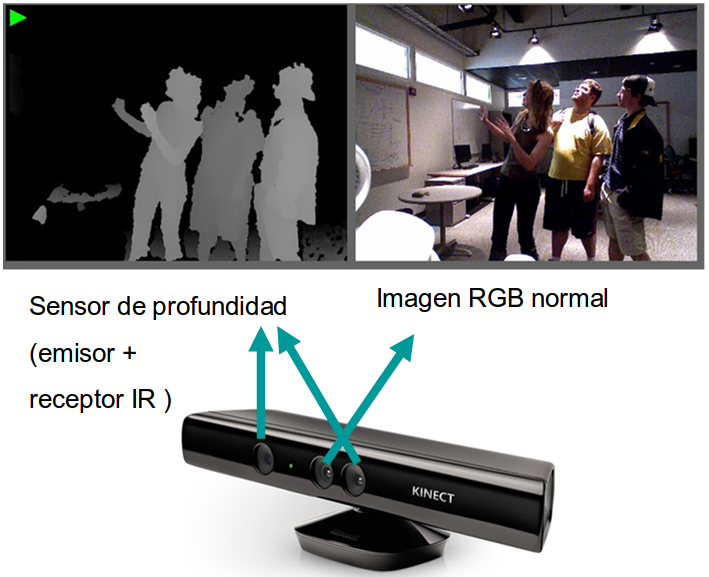
\includegraphics[scale=0.6]{db/kinect1}
\end{center}

\end{myframe}

\begin{myframe}
\frametitle{Kinect SDK}
\begin{center}
  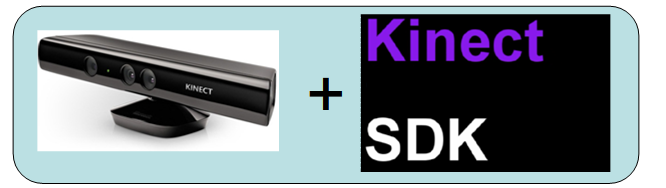
\includegraphics[scale=0.52]{db/kinectsdk} \\
  {\huge \textbf{=}} \\
  \begin{columns}
  \begin{column}{0.7\textwidth}
    \centering
    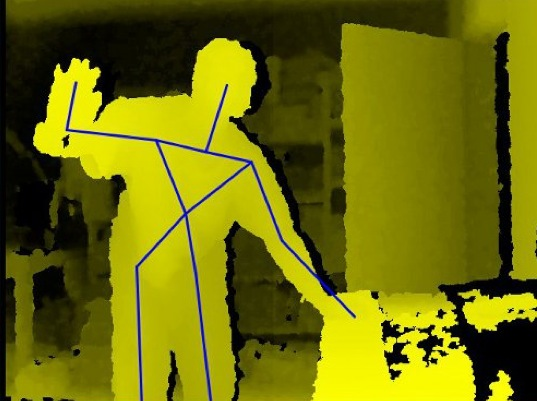
\includegraphics[width=0.9\textwidth]{db/skeleton2}
  \end{column}
  \begin{column}{0.3\textwidth}
      \centering
      \vspace{-20pt}
      \blockitemize{}{
      \item Hasta 5 personas
      \item Tiempo real, 30 fps
      \item Coordenadas espacio 3D
      \item Posición 20 articulaciones
      }
  \end{column}
  \end{columns}
\end{center}
\end{myframe}

\subsection{Bases de datos}

\begin{myframe}
\frametitle{Base de datos LNHG}
\centering
\begin{block}{}
\centering
720 gestos \hspace{1em} 36 clases \hspace{1em} 20 ejemplares por clase
\end{block}
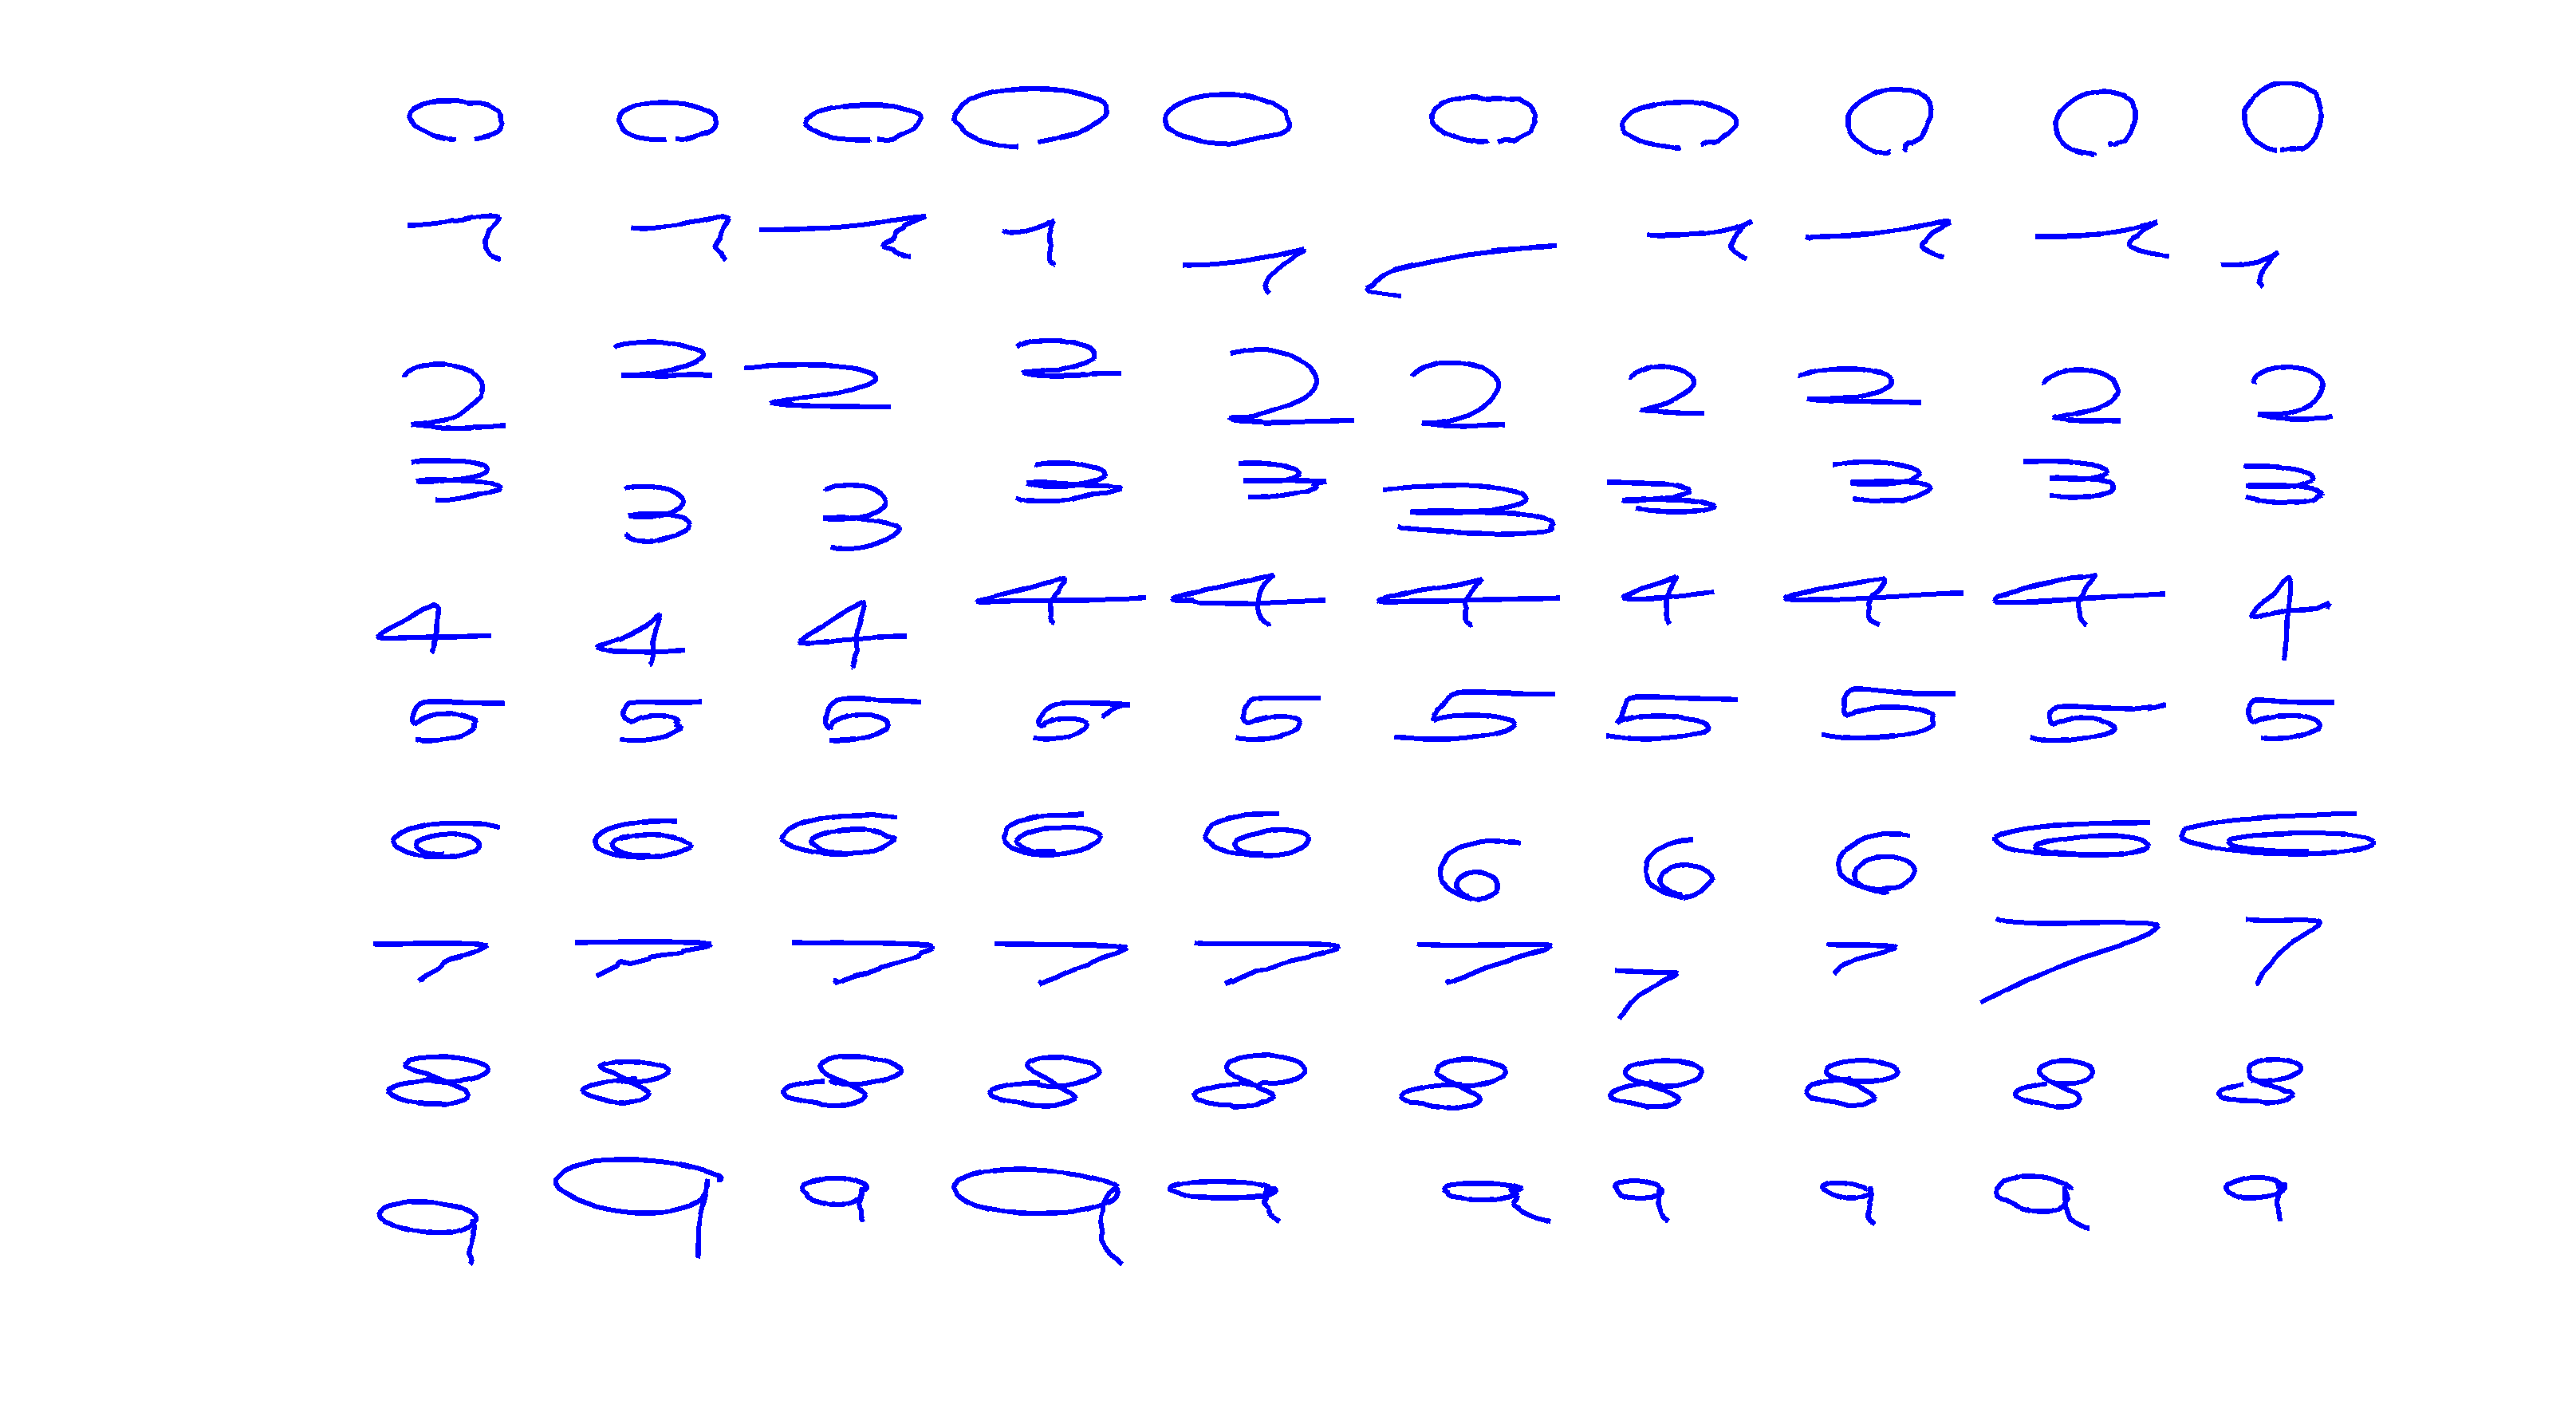
\includegraphics[scale=0.15]{db/segmented_all}\\
(Proyecciones en el plano $X-Y$)

\end{myframe}

%\begin{myframe}
%\frametitle{Base de datos Celebi2013 (ajena) }
%\centering
%\begin{block}{}
%\centering
%224 gestos \hspace{2em} 8 clases \hspace{2em} 20+8 ejemplares por clase \\
%\end{block}
%
%\begin{block}{}
%\centering
%Empuje hacia abajo, arriba, saludo y movimientos izq-der
%\end{block}
%
%
%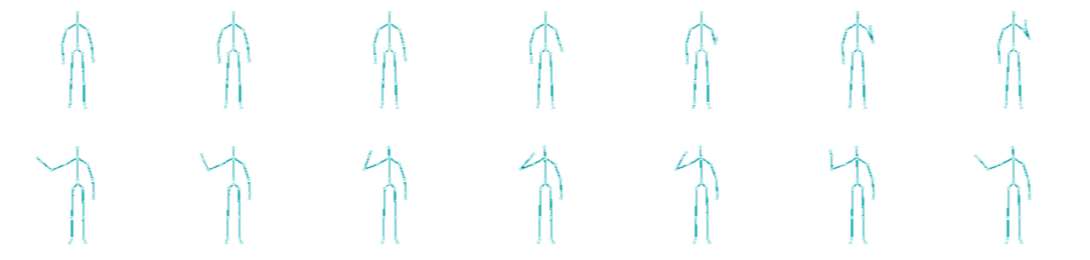
\includegraphics[scale=0.5]{db/celebi}\\
%(Proyecciones en el plano $X-Y$)
%
%\begin{alertblock}{Advertencia}
%\begin{itemize}
%\centering
%\item 8 clases = 4 tipos de gesto, con manos distintas \\
%\item Yo considero 4 clases
%\end{itemize}
%\end{alertblock}
%\end{myframe}

\begin{myframe}

\frametitle{Preprocesamiento y Representación}
\esquemaaprendizajepreprocesamiento{0.5}
%\esquemaavalidacionpreprocesamiento{0.4}
\end{myframe}

\subsection{Preprocesamiento y Representación}

\begin{myframe}
\frametitle{Modelo de gestos}
\centering
\begin{block}{}
\centering
Gesto = Trayectoria en el espacio virtual
\end{block}
Invariante a:

\begin{tabular}{C{0.5\linewidth}C{0.5\linewidth}}


   \frame{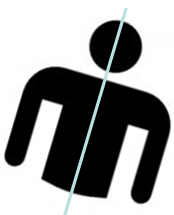
\includegraphics[width=0.20\textwidth]{db/rotation1}}
   \frame{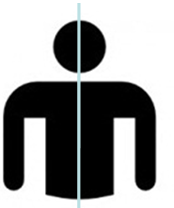
\includegraphics[width=0.20\textwidth]{db/rotation2}}
   &        
  \frame{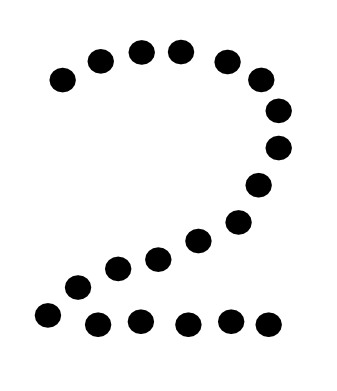
\includegraphics[width=0.20\textwidth]{features/gesture_slow}}
  \frame{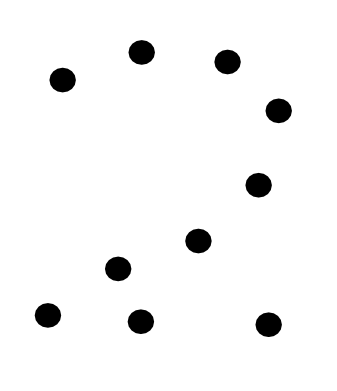
\includegraphics[width=0.20\textwidth]{features/gesture_fast}} \\
    Rotación del usuario & Velocidad \\
  \frame{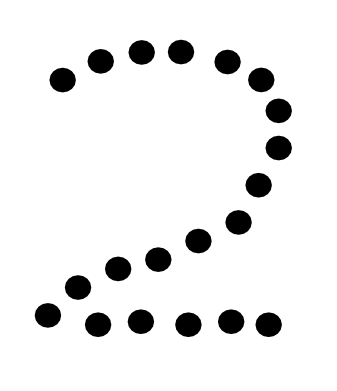
\includegraphics[width=0.20\textwidth]{features/gesture}}
  \frame{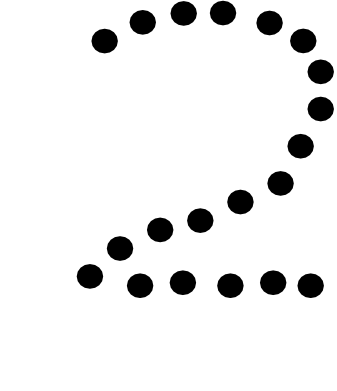
\includegraphics[width=0.20\textwidth]{features/gesture_traslation}}
   &
  \frame{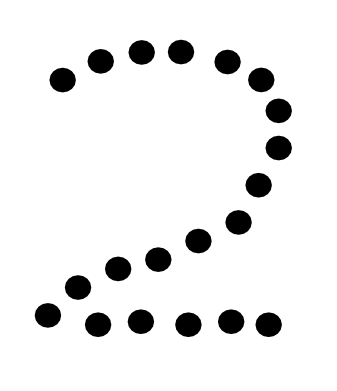
\includegraphics[width=0.20\textwidth]{features/gesture}}
  \frame{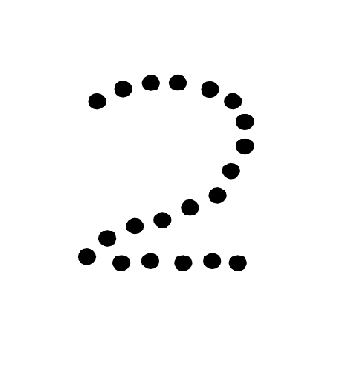
\includegraphics[width=0.20\textwidth]{features/gesture_scale}}
   \\
   Traslación & Escala 
\end{tabular}

\end{myframe}



\begin{myframe}
\frametitle{Preprocesamiento: Rotación}
\begin{center}
  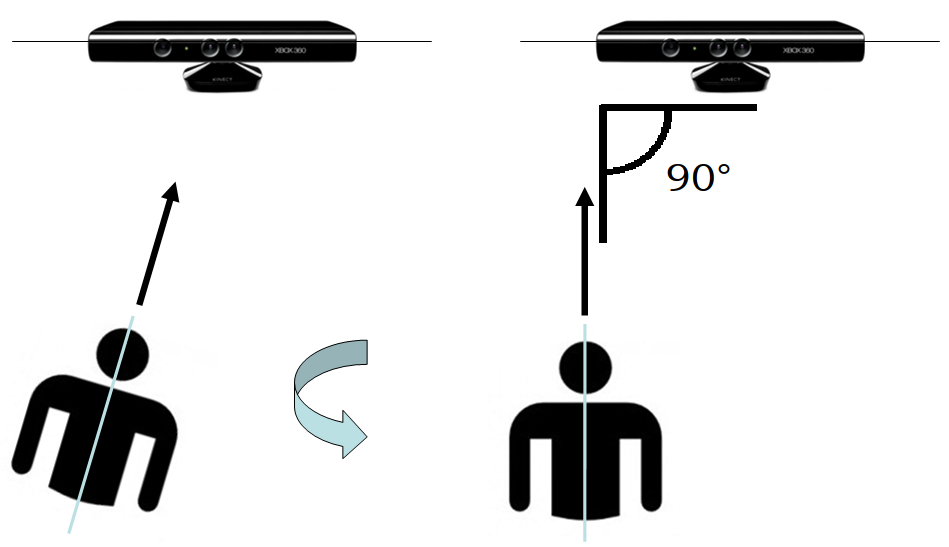
\includegraphics[scale=0.6]{db/rotation}
\end{center}
\end{myframe}

\begin{myframe}
\frametitle{Pre: Suavizado y re-muestreo $\rightarrow$ Invariancia a velocidad}
\begin{center}
  Original  \hspace{55pt}  Suavizado \hspace{45pt} Re-muestreo \\ 
  \hspace{80pt}  (Moving average) \hspace{28pt} (n posiciones) \\ 
  \vspace{10pt}
  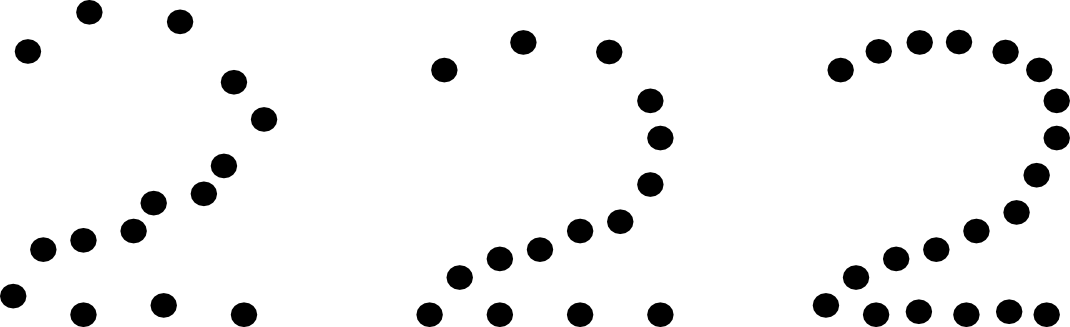
\includegraphics[scale=1.5]{features/preprocesamiento2}
\end{center}

\begin{block}{Ejemplo de re-muestreo con $n=6$}
\begin{itemize}
\item Longitud de arco $L=10$.
\item Nuevos puntos de muestreo: $d_k=Lk/(n-1)=10k/5=2k$ $k=0,\dots,(n-1)$. ($d=0,2,4,6,8,10$)
\item Calcular el punto a distancia $d_k$ del principio, interpolando.
\end{itemize}
\end{block}
\end{myframe}


\begin{myframe}
\frametitle{Representacion: Secuencia de Direcciones}
\begin{center}
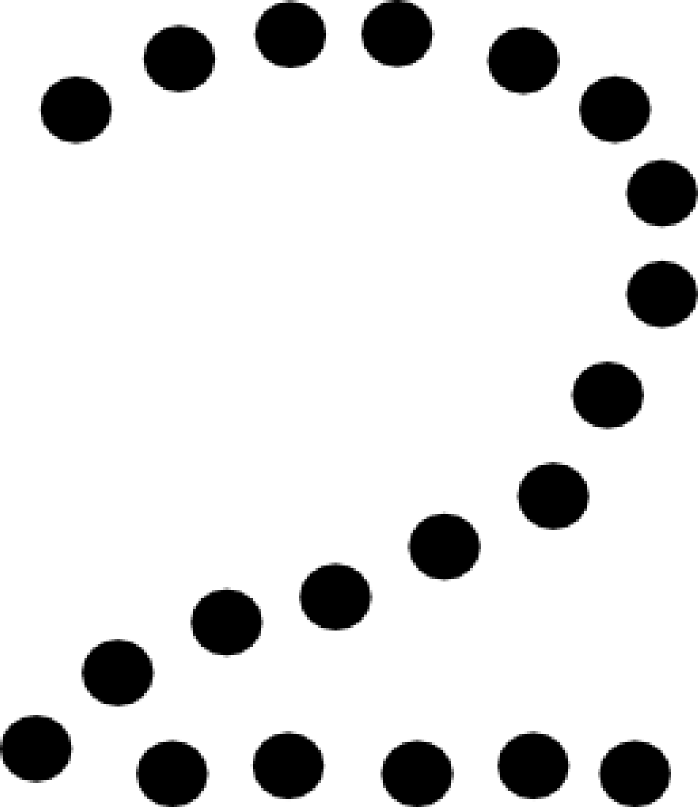
\includegraphics[scale=0.6]{features/el2} \\
\vspace{7pt}
 Primera diferencia \arrowdown ($\mathbf{d}= \mathbf{g}[n+1] - \mathbf{g}[n] $) $\rightarrow$ Invariancia a la traslación \\
\vspace{5pt}
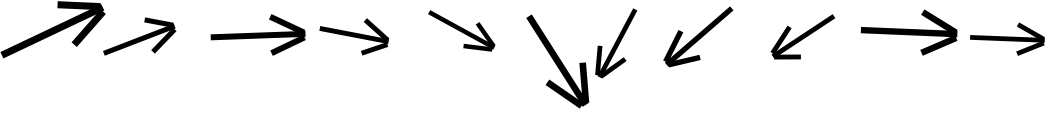
\includegraphics[scale=0.51]{features/first_difference}\\
\vspace{5pt}
 Normalización  \arrowdown ($||\mathbf{d}||=1$) $\rightarrow$ Invariancia a la escala\\
\vspace{5pt}
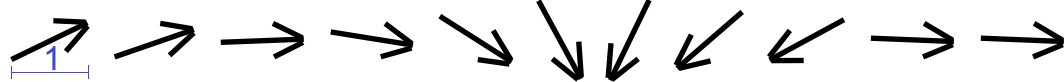
\includegraphics[scale=0.51]{features/features_normalized}
\end{center}

\end{myframe}
